%%%%%%%%%%%%%%%%%%%%%%%%%%%%%%%%%%%%%%%%%
% APA Assignment Article
% LaTeX Template
% Version 2.0 (February 7, 2023)
%
% This template originates from:
% https://www.LaTeXTemplates.com
%
% Author:
% Vel (vel@latextemplates.com)
%
% License:
% CC BY-NC-SA 4.0 (https://creativecommons.org/licenses/by-nc-sa/4.0/)
%
% NOTE: The bibliography needs to be compiled using the biber engine.
%
%%%%%%%%%%%%%%%%%%%%%%%%%%%%%%%%%%%%%%%%%

%----------------------------------------------------------------------------------------
%	PACKAGES AND OTHER DOCUMENT CONFIGURATIONS
%----------------------------------------------------------------------------------------

\documentclass[
	letterpaper, % Paper size, use either a4paper or letterpaper
	10pt, % Default font size, can also use 11pt or 12pt, although this is not recommended
	unnumberedsections, % Comment to enable section numbering
	twoside, % Two side traditional mode where headers and footers change between odd and even pages, comment this option to make them fixed
]{APAAssignment}

\addbibresource{bibliography.bib} % BibLaTeX bibliography file

\runninghead{MICS CYBER 252, Fall-2024 Hands On Lab Unit 10} % A shortened article title to appear in the running head, leave this command empty for no running head

\footertext{\textit{Hands On Lab 10} (MICS CYBER 252, Fall -2024)} % Text to appear in the footer, leave this command empty for no footer text

\setcounter{page}{1} % The page number of the first page, set this to a higher number if the article is to be part of an issue or larger work

%----------------------------------------------------------------------------------------
%	TITLE SECTION
%----------------------------------------------------------------------------------------

\usepackage[title,toc,titletoc]{appendix}
\usepackage{titlesec}
\usepackage{lscape}
\usepackage{fontawesome}

\title{Hands On Lab: Unit 10 \\ MICS-252, Fall 2024 \\ Incident Response, Linux} % Article title, use manual lines breaks (\\) to beautify the layout

% Authors are listed in a comma-separated list with superscript numbers indicating affiliations
% \thanks{} is used for any text that should be placed in a footnote on the first page, such as the corresponding author's email, journal acceptance dates, a copyright/license notice, keywords, etc
% Affiliations are output in the \date{} command
\date{UC Berkeley School of Information \\
MICS Course 252 Fall 2024 (Kristy Westphal)
}


\author{
	Prepared by: Karl-Johan Westhoff \\
	email: \href{mailto:kjwesthoff@berkeley.edu}{kjwesthoff@berkeley.edu}
}


% % Full-width abstract
% \renewcommand{\maketitlehookd}{%
% 	\begin{abstract}
% 		\noindent Lorem ipsum dolor sit amet,rta porttitor.
% 	\end{abstract}
% }

%----------------------------------------------------------------------------------------

\setcounter{tocdepth}{5}
\setcounter{secnumdepth}{5}
\usepackage[title]{appendix}

\begin{document}
\onecolumn
\maketitle % Output the title section

%----------------------------------------------------------------------------------------
%	ARTICLE CONTENTS
%----------------------------------------------------------------------------------------


\section{Introduction}
We are given a snapshot of some files from a Linux host which has been compromised.
Linux version 7.1 is mentioned, assuming this means the Red Hat Distribution 7.1, code named "Seawolf", released in 2001 \cite{RedHatOnWIki}

\section{Look at the files}
It looks like we were issued the contents of Linux system 'var' folder (or parts thereof). In Linux the /var folder contains variable data files. This includes spool directories and files, administrative and logging data, and transient and temporary files \cite{VarFolder}. Folder content is shown in Figure \ref{fig:givenFiles}

\begin{figure}[!htp] % Single column :figure	
	\centering
	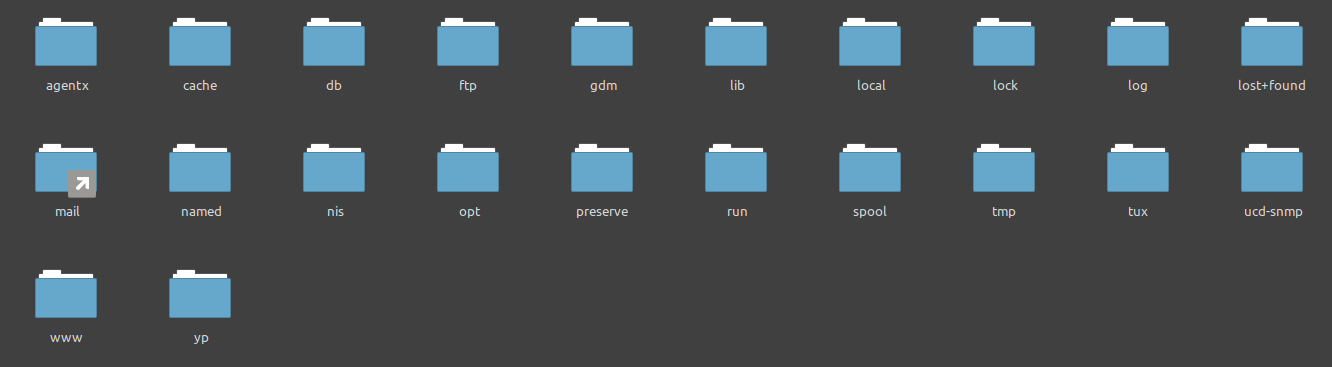
\includegraphics[width=0.75\linewidth]{givenFiles_var.png}
	\caption{We are given the 'var' folder from a compromised Linux host}
	\label{fig:givenFiles}
\end{figure}

\subsection{/tmp folder}
An interesting folders is the /tmp folder holding temporary files. The /tmp folder could contain artifacts from someone trying privilege escalation or achieve persistence. Sometimes un-careful design of by user privileged sudo executable files may contain relative links to files which are then executed with sudo privilege, and a /tmp folder is a good place to execute these. But the /tmp folder is empty.

\subsection{/www folder}
The /www folder indicates a web server was installed on the compromised host, this could be an attack vector. Sure enough poking around the html files installed by various modules in the web app, the following was enumerated:

\begin{itemize}
	\item Apache version 1.3b5 is used (html/manual/mod/mod\_perl.html)
	\item mod\_ssl version 2.8 is used to manage the server via SSL v2/v3 and TLS v1 implemented using openSSL (html/manual/mod/mod\_ssl/index.html)
	\item uses s php-nuke Version from 2003 to handle database transactions to a mySQL database
\end{itemize}


The modules and versions of the installed web server are outdated and expose multiple vulnerabilities: XSS, remote code execution, SQL injection \cite{Apache1.3Vulnerabilities}. \\

It is not stated if the compromised Linux host functioned as a webserver, or even if the web server was operating at the time of breach. Will look for evidence in the further analyses.

\subsection{/log folder}
The log folder has the following sub folders:
\begin{itemize}
	\item httpd: Apache webserver log files, contains time stamped access and error log entries
	\item news: no content
	\item sa: may hold "system activity" logs, has a limited number of binary files and some HH:MM:SS time stamped entries
	\item samba: Indicates that a SMB file service (Interface to Windows files sharing protocol) has been running. The logs contain some time stamped "authentication failed" entries and connection reset entries. These could be correlated with other events based on timestamp
	\item squid: logs for a caching proxy used with the web server (indicating that the compromised host was deployed as a web server - you would not need caching for a test/small number of user application) Holds time stamped logs showing failed http requests etc.
	\item vbox: empty
\end{itemize}

The log folder holds a number of species of log files, split into multiple files, some of which are empty:

\begin{itemize}
	\item boot.log.x (1-25): Logging startup, could show artifacts of malicious persistence on the host
	\item cron.x (1-25): Logs scheduled jobs, definitely a place to look for persistence attempts
	\item dmesg: Kernel stuff, may capture things during boot before other services come online
	\item lastlog: Binary
	\item maillog (1-25): Logs for mail-server (apparently the thing also served mail..)
	\item messages (1-25): Messages from various services (syslog, ftp etc)
	\item mysqld.log(1-25): Not much here, most of the files are empty
	\item pacct (1-6): Binary files, containing information on user's command execution
	\item secure (1-25): Authentication events (logins, ssh etc.)
	\item spooler (1-25): Empty
	\item tmplog: Looks like a mashup of different files
	\item wtmp (1): Binary
	\item xferlog (1-24): Empty
\end{itemize}

\section{The log files}
Just looking at the files, the "secure" logs, containing login attempts and the "cron" logs containing persistently scheduled jobs look the most interesting. The logs show some authentication attempts that failed.\\
I decided to explore all the files, looking for keywords indicating failed login attempts, tool of choice: bash and grep (see Appendix \ref{app:process}) for some notes on the process of choosing tools..

\begin{verbatim}
	grep -Ei 'fail*|illegal|unauth*|refused' {messages*,secure*,boot*,dmesg*,cron*}
\end{verbatim}

Gives a long list of failed login attempts, further reducing this to get a list of unique users and ip addresses repeatedly trying to login,
piping (|) the previous result to a regex searching for IP addresses:
\subsection{Suspicious IP's}
\begin{verbatim}
grep -E -o '(25[0-5]|2[0-4][0-9]|[01]?[0-9][0-9]?)\.(25[0-5]|2[0-4][0-9]|[01]?[0-9][0-9]?)
\.(25[0-5]|2[0-4][0-9]|[01]?[0-9][0-9]?)\.(25[0-5]|2[0-4][0-9]|[01]?[0-9][0-9]?)'
\end{verbatim}

And sorting by unique occurrences and counting the attempts:

\begin{verbatim}
	 | sort | uniq -c | sort -nr
\end{verbatim}

Gives a list of 'candidates' with a high number of failed attempts to log in Figure \ref{fig:ipShortList} (full list shown in Appendix \ref{app:numberedFailedLogons}):

\begin{figure}[!htp] % Single column :figure	
	\centering
	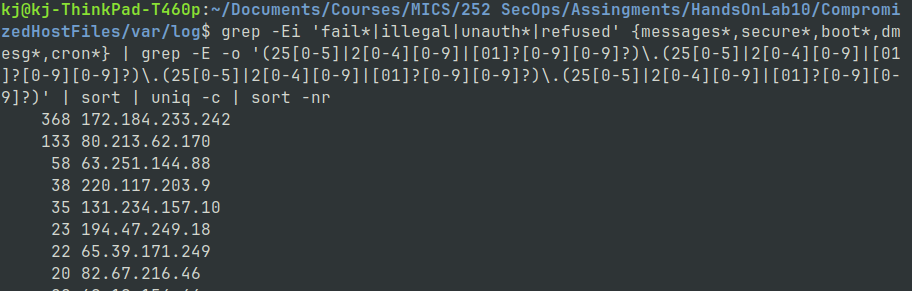
\includegraphics[width=0.75\linewidth]{ipShortList.png}
	\caption{IP's sorted by failed login attempts, complete list in Appendix \ref{app:numberedFailedLogons}}
	\label{fig:ipShortList}
\end{figure}

\subsubsection{"172.184.233.242"}
has 368 failed attempts and seems to be associated with the domain "acb8e9f2.ipt.aol.com", grepping for that gives a long list of failed FTP logons. Trying to see if it was successful at some point

A bunch of ftp sessions in the "secure" logs show as started, the logs show File:Date Time Host (ns1) service(xinetd)[pid,704] protocol(ftp), xinetd pid and source IP
\begin{figure}[!htp] % Single column :figure	
	\centering
	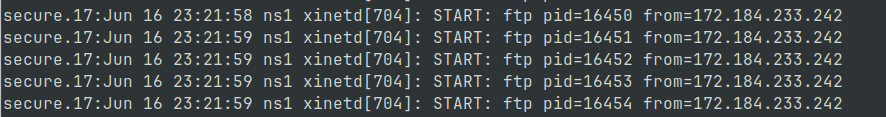
\includegraphics[width=\linewidth]{secure17ftp.png}
	\caption{FTP processes attempted starts}
	\label{fig:secure17ftp}
\end{figure}

They all seem to be short duration, 45-65s (matching START and EXIT for each pid) seconds indicating they were refused by the server, so nothing conclusive, other that a lot of FTP logon attempts from the source.


\subsubsection{"80.213.62.170"}
has 133 failed logins trying to access an SSH service, but is unsuccessful, looks like a failed credential spraying attempt.

\subsubsection{"Remaining candidates"}
The rest of the ip's with failed logon attempts in Figure \ref{fig:ipShortList} are related to failed ssh logons.


\subsection{grep'ing for ssh}
grep and filtering out all the rejected logon attempts:

\begin{verbatim}
	grep -Ei 'sshd' {messages*,secure*,boot*,dmesg*,cron*}
	| grep -E -v -i 'fail*|clos*|disconn*|reverse*|did*|illegal'
\end{verbatim}
Shows that some IP's are scanning the ssh server using "SSH-1.0-SSH\_Version\_Mapper .  Don't panic." again this could indicate someone poking  around. Checking for successful logons next:

\begin{verbatim}
	grep -Ei 'sshd' {messages*,secure*,boot*,dmesg*,cron*} | grep -E -i accepted
\end{verbatim}

Shows that only the user 'test' has been able to log in, and making a unique list of the IP's, see Figure \ref{fig:successfulSSH} narrows it down to a list that can be compared to the sources with many failed logons:


\begin{figure}[!htp] % Single column :figure	
	\centering
	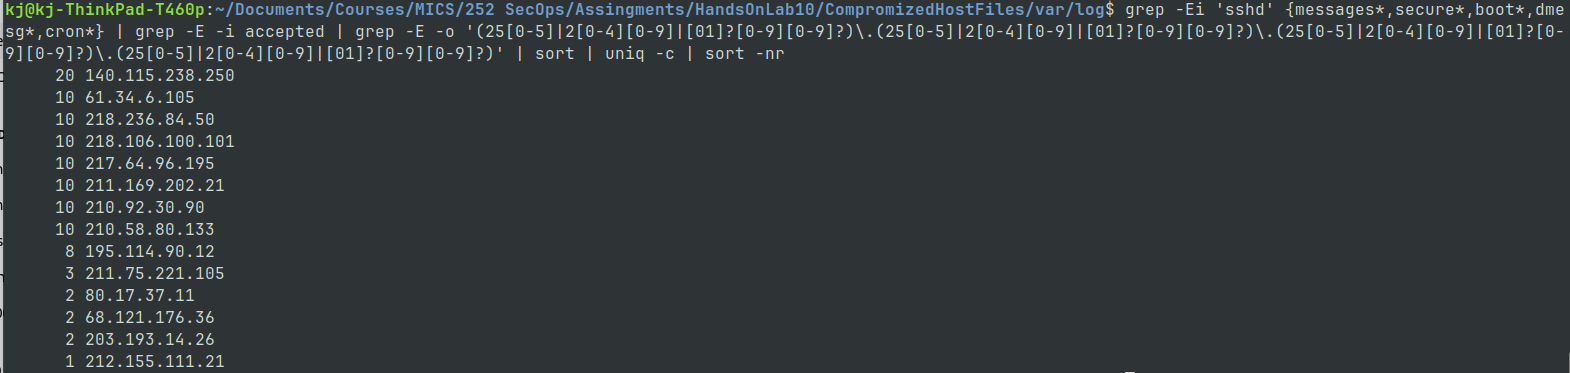
\includegraphics[width=\linewidth]{SuccessfulSSHlogins.png}
	\caption{List of IP's that have successfully logged in}
	\label{fig:successfulSSH}
\end{figure}

The successful logins, which also have failed attempts are:
\begin{verbatim}
	218.106.100.101 (10 failed attepmts)
	212.155.111.21 (4 failed attempts, looks like a forgotten password)
\end{verbatim}

218.106.x... has 10 failed logon attempts, will look into what else that host has been up to. The IP has 10 failed attempts on September 27, but manages to log in on October 7. All attempts are in quick succession spanning a few seconds, looks automated see Figure \ref{fig:AutomatedLogons}

\begin{figure}[!htp] % Single column :figure	
	\centering
	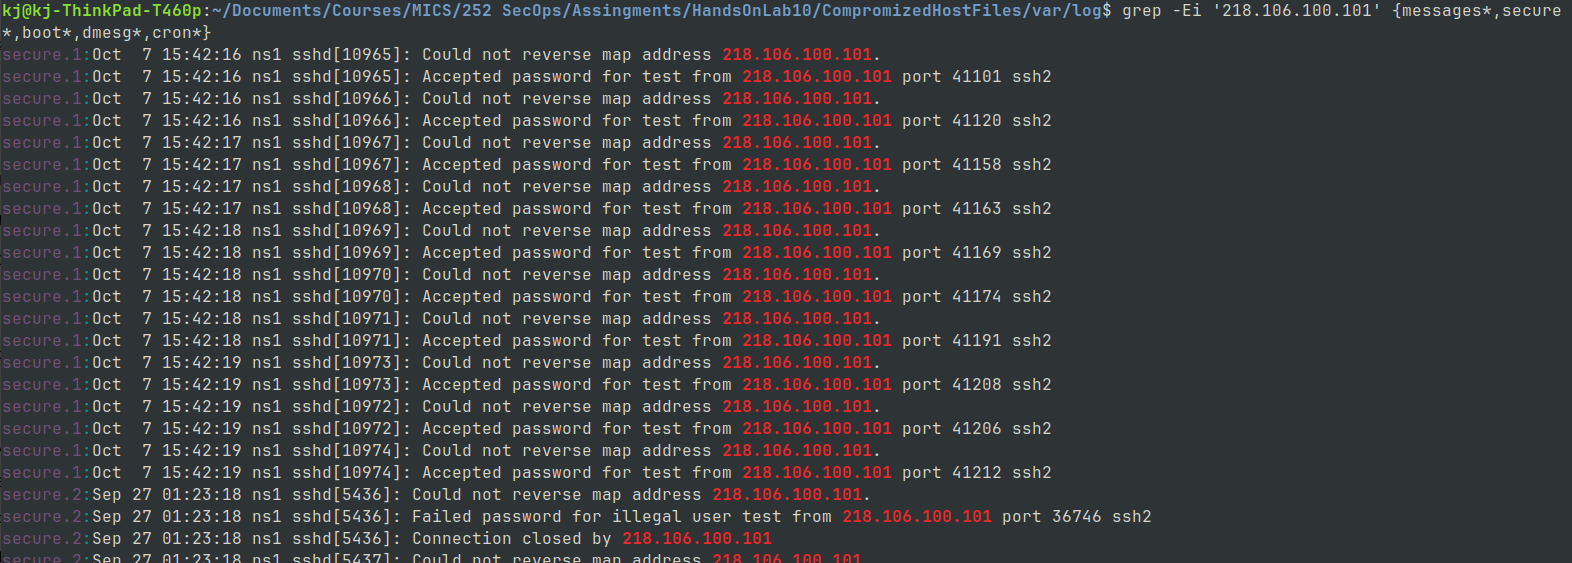
\includegraphics[width=\linewidth]{AutomatedLogons.png}
	\caption{218.106.100.101 successful logons, multiple ssh processes in quick succession}
	\label{fig:AutomatedLogons}
\end{figure}





\section{Conclusion}
The ssh logons from 218.106.100.101 look suspicious, the cron logs however, did not show signs of persistence. Next step would be to look at the pacct logs which are in binary (will require a tool for reading). For now I think 218.106.100.101, posing a user 'test' is the culprit. Determining if the Apache web server was the initial attack vector can be determined by looking for reverse shell commands being executed, this may be found in the pacct logs, I was unable to find logs for the Apache server and grepping for reverse shell execution (bash -i >\&) did not reveal anything. The attack uses password spraying and automated (fast) logon attempts, in the IDS limiting the number of and frequency of failed password attempts could easily alert or block the attempts. For now 218.106.100.101 should be investigated further..



\printbibliography % Output the bibliography   

%----------------------------------------------------------------------------------------



%----------------------------------------------------------------------------------------
%	 Appendices
%----------------------------------------------------------------------------------------
%
%\appendix


\clearpage
\chapter{Appendices}
\begin{appendices}

	\section{IP's with failed logins}\label{app:numberedFailedLogons}
	\begin{verbatim}
		grep -Ei 'fail*|illegal|unauth*|refused' {messages*,secure*,boot*,dmesg*,cron*} 
		| grep -E -o '(25[0-5]|2[0-4][0-9]|[01]?[0-9][0-9]?)\.(25[0-5]|2[0-4][0-9]|[01]?[0-9][0-9]?)
		\.(25[0-5]|2[0-4][0-9]|[01]?[0-9][0-9]?)\.(25[0-5]|2[0-4][0-9]|[01]?[0-9][0-9]?)' 
		| sort | uniq -c | sort -nr



    368 172.184.233.242
    133 80.213.62.170
     58 63.251.144.88
     38 220.117.203.9
     35 131.234.157.10
     23 194.47.249.18
     22 65.39.171.249
     20 82.67.216.46
     20 69.19.154.44
     20 64.246.58.96
     20 61.211.237.34
     20 219.94.51.51
     20 218.104.55.15
     20 212.40.162.195
     20 211.180.157.251
     20 211.174.186.145
     19 65.194.200.129
     19 210.0.186.83
     17 217.172.188.217
     11 61.41.235.53
     11 211.114.173.193
     10 80.237.77.94
     10 70.240.3.138
     10 67.18.172.10
     10 64.140.42.69
     10 61.166.155.162
     10 219.113.213.21
     10 218.30.21.236
     10 218.158.126.247
     10 218.106.100.101
     10 213.232.127.249
     10 210.114.220.147
     10 196.40.45.116
     10 196.35.68.95
     10 163.180.21.201
     10 153.104.6.221
      9 61.166.6.60
      9 224.0.1.1
      9 220.92.31.135
      9 203.72.251.14
      9 195.78.43.183
      9 193.96.238.131
      6 69.0.134.72
      6 62.179.22.250
      6 203.71.62.9
      4 212.155.111.21
      4 211.240.65.3
      2 61.221.77.82
      2 220.168.17.55
      2 216.234.56.11
      1 65.104.169.18
      1 62.204.197.193
      1 62.166.92.73
      1 212.118.103.2
      1 211.117.191.70
      1 210.83.203.34
      1 210.112.147.22
      1 142.207.115.6

	\end{verbatim}

	\section{A bit on my process working on this}\label{app:process}
	My initial idea was to use this assignment to explore a new log analysis tool, so I installed "The Sleuth Kit" and Autopsy. That took quite some time and the results were inconclusive...\\

	Then I thought 'pandas' in python using 'glob' would be a good fit, easy graphics to see what is going on etc.. But pandas is slow going and not ideal for working with many different kinds of log files.. it was taking too long I was running out of time. \\

	So I decided to poke around the data using grep and awk. It proved to be, by far the quickest and also the most intuitive

\end{appendices}
\end{document}
